\documentclass[border=3pt,tikz]{standalone}
\usepackage{physics}
\usepackage{tikz}
\usepackage[outline]{contour} % glow around text
\usetikzlibrary{calc}
\usetikzlibrary{angles,quotes} % for pic
\usetikzlibrary{arrows.meta}
\usetikzlibrary{patterns}
\usetikzlibrary{bending} % for arrow head angle
\tikzset{>=latex} % for LaTeX arrow head
\contourlength{0.8pt}

\colorlet{xcol}{blue!70!black}
\colorlet{myred}{red!65!black}
\tikzstyle{rvec}=[->,xcol,very thick,line cap=round]
\tikzstyle{mass line}=[line width=0.5,draw=red!30!black]
\tikzstyle{myarr}=[-{Latex[length=3,width=2]},blue!40!black]
\tikzstyle{myarr2}=[{Latex[length=3,width=2]}-{Latex[length=3,width=2]},blue!40!black]
\tikzstyle{mass}=[mass line, top color=red!40!black!30,bottom color=red!40!black!10,shading angle=30]
\tikzstyle{middle mass}=[mass line,top color=red!40!black!50,bottom color=red!40!black!50, middle color=red!40!black!10,shading angle=30]

\def\r{0.05} % pulley small radius
\tikzset{
	pics/rotarr/.style={
		code={
			\draw[white,line width=0.8] ({#1*cos(210)},0) arc(-210:35:{#1} and {0.35*#1});
			\draw[-{>[flex'=1]}] ({#1*cos(210)},0) coordinate (W1) arc(-210:35:{#1} and {0.35*#1})
			node[midway] (W2) {} --++ (150:0.1) coordinate (W3);
	}},
	pics/rotarr/.default=0.3,
}

\begin{document}
	
	% MOMENT OF INERTIA - HOLLOW CYLINDER
	\def\H{1.6}   % cylinder length
	\def\Rx{0.70} % horizontal radius
	\def\Ry{0.20} % vertical radius
	\def\sx{0.88}
	\def\sy{0.75}
	\def\ang{-30} % angle of whole picture

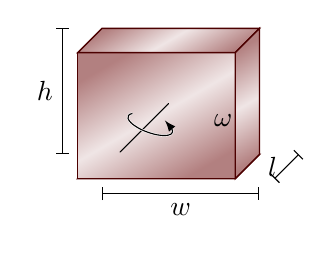
\begin{tikzpicture}
	\def\w{2.0}   % width
	\def\h{1.6}   % height
	\def\l{0.8}   % length
	\def\ang{-20} % angle of whole picture
	\coordinate (O) at (0,0,0); % Central point
	
	% Draw the box
	\fill[mass] (0,0,0) --++ (\w,0,0) --++ (0,\h,0) --++ (-\w,0,0) -- cycle;
	% Sides
	\fill[mass] (0,0,0) --++ (\w,0,0) --++ (0,0,\l) --++ (-\w,0,0) -- cycle; % bottom


		% Front face

	% Back face
	\fill[middle mass] (0,0,\l) --++ (\w,0,0) --++ (0,\h,0) --++ (-\w,0,0) -- cycle;
	%\fill[middle mass] (0,0,0) --++ (0,0,\l) --++ (0,\h,0) --++ (0,-\h,0) -- cycle; % left
	\fill[middle mass] (0,\h,0) --++ (\w,0,0) --++ (0,0,\l) --++ (-\w,0,0) -- cycle; % top
	\fill[middle mass] (\w,0,0) --++ (0,0,\l) --++ (0,\h,0) --++ (0,0,-\l) -- cycle; % right

		
	% Draw the axis through the center
	\draw[line cap=round] (0.5*\w,0.5*\h,0.5*\l) -- (0.5*\w,0.5*\h,2.5*\l);
	\pic[xscale=1,rotate=\ang] at (0.5*\w,0.5*\h,1.2*\l) {rotarr};
	\node[right=0.5cm] at (W3) {$\omega$};
	
	% Labeling the dimensions
	\draw[|-|, yshift=-0.5cm] (0,0,0) --++ (\w,0,0) node[midway, below] {$w$};
	\draw[|-|, xshift=-0.5cm] (0,0,0) --++ (0,\h,0) node[midway, left] {$h$};
	\draw[|-|, xshift=2.5cm, yshift=0cm] (0,0,0) --++ (0,0,\l) node[midway, left] {$l$};
\end{tikzpicture}



\end{document}